\AppendixChapter{Caracterización}

\section{Entrevista estructurada}
\label{sec:entrevista}

En esta sección se presenta la entrevista estructurada completa aplicada al grupo de investigación.

% --- PÁGINAS DEL PDF INCLUIDAS INDIVIDUALMENTE COMO FIGURAS ---
\begin{figure}[H]
	\centering
	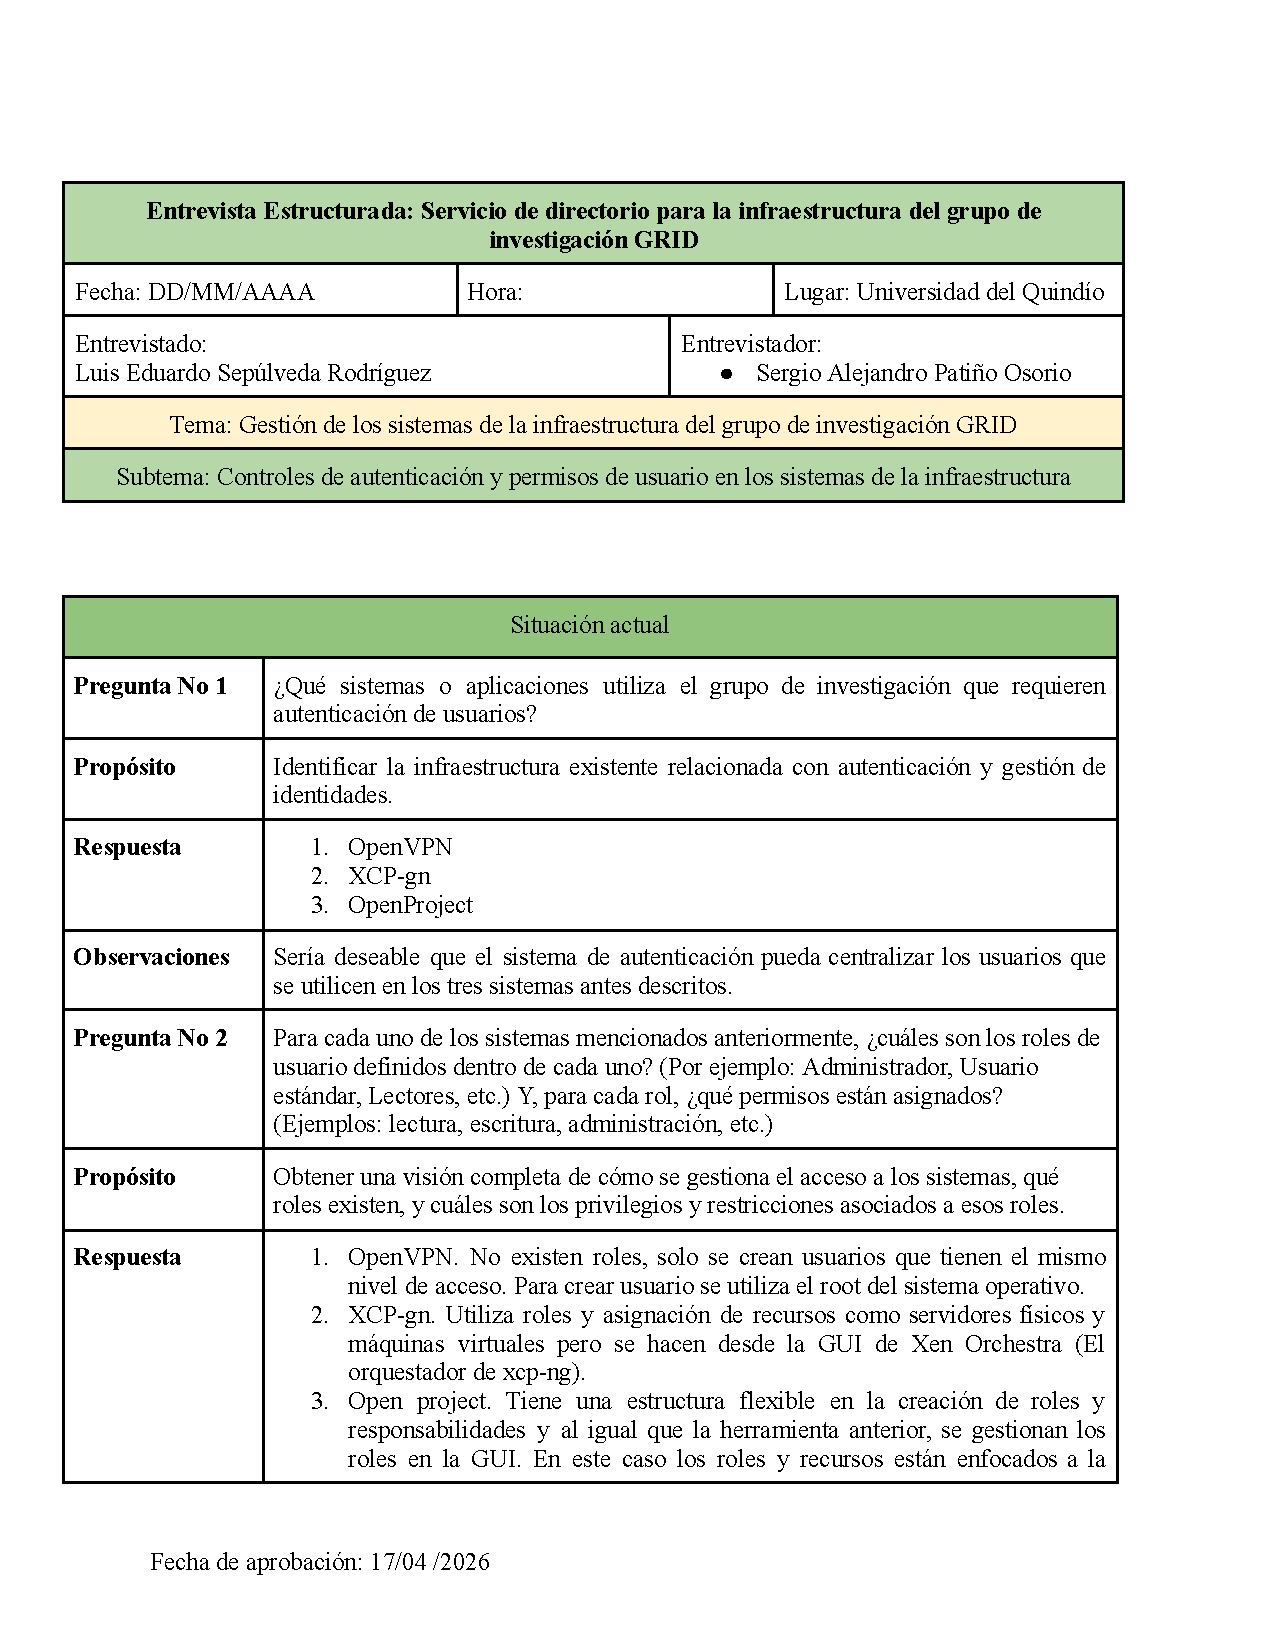
\includegraphics[page=1, width=\textwidth, height=0.9\textheight, keepaspectratio]{backmatter/apendices/entrevista/imagenes/entrevista.pdf}
	\caption{Entrevista estructurada -- Página 1}
	\label{fig:entrevista_p1}
\end{figure}

\begin{figure}[H]
	\centering
	\includegraphics[page=2, width=\textwidth, height=0.9\textheight, keepaspectratio]{backmatter/apendices/entrevista/imagenes/entrevista.pdf}
	\caption{Entrevista estructurada -- Página 2}
	\label{fig:entrevista_p2}
\end{figure}

\begin{figure}[H]
	\centering
	\includegraphics[page=3, width=\textwidth, height=0.9\textheight, keepaspectratio]{backmatter/apendices/entrevista/imagenes/entrevista.pdf}
	\caption{Entrevista estructurada -- Página 3}
	\label{fig:entrevista_p3}
\end{figure}

\begin{figure}[H]
	\centering
	\includegraphics[page=4, width=\textwidth, height=0.9\textheight, keepaspectratio]{backmatter/apendices/entrevista/imagenes/entrevista.pdf}
	\caption{Entrevista estructurada -- Página 4}
	\label{fig:entrevista_p4}
\end{figure}

\begin{figure}[H]
	\centering
	\includegraphics[page=5, width=\textwidth, height=0.9\textheight, keepaspectratio]{backmatter/apendices/entrevista/imagenes/entrevista.pdf}
	\caption{Entrevista estructurada -- Página 5}
	\label{fig:entrevista_p5}
\end{figure}
